% Exemplo de relatório técnico do IC
% Criado por P.J.de Rezende antes do Alvorecer da História.
% Modificado em 97-06-15 e 01-02-26 por J.Stolfi.
% Last edited on 2003-06-07 21:12:18 by stolfi

% modificado em 1o. de outubro de 2008
\documentclass[11pt,twoside]{article}
\usepackage{techrep-ic}

%%% SE USAR INGLÊS, TROQUE AS ATIVAÇÕES DOS DOIS COMANDOS A SEGUIR:
\usepackage[brazil]{babel}
%% \usepackage[english]{babel}

%%% SE USAR CODIFICAÇÃO LATIN1, TROQUE AS ATIVAÇÕES DOS DOIS COMANDOS A
%%% SEGUIR:
%% \usepackage[latin1]{inputenc}
\usepackage[utf8]{inputenc}
\usepackage{graphicx}
\usepackage{url}
\usepackage{multirow}
\usepackage{multicol}
\usepackage{amsmath}
\usepackage{upgreek}
\usepackage{caption}
\usepackage{subcaption}

\bibliographystyle{abbrv}

\begin{document}

%%% PÁGINA DE CAPA %%%%%%%%%%%%%%%%%%%%%%%%%%%%%%%%%%%%%%%%%%%%%%%
% 
% Número do relatório
\TRNumber{???}

% DATA DE PUBLICAÇÃO (PARA A CAPA)
%
\TRYear{12}  % Dois dígitos apenas
\TRMonth{11} % Numérico, 01-12

% LISTA DE AUTORES PARA CAPA (sem afiliações).
\TRAuthor{R. Barboza Jr \and D. C. S. Lucas \and A. S. Ferreira}

% TÍTULO PARA A CAPA (use \\ para forçar quebras de linha).
\TRTitle{Uma Análise Comparativa Entre o Desempenho de Máquinas Virtuais
  Interpretadas de Sistema e de Processo}

\TRMakeCover

%%%%%%%%%%%%%%%%%%%%%%%%%%%%%%%%%%%%%%%%%%%%%%%%%%%%%%%%%%%%%%%%%%%%%%
% O que segue é apenas uma sugestão - sinta-se à vontade para
% usar seu formato predileto, desde que as margens tenham pelo
% menos 25mm nos quatro lados, e o tamanho do fonte seja pelo menos
% 11pt. Certifique-se também de que o título e lista de autores
% estão reproduzidos na íntegra na página 1, a primeira depois da
% página de capa.
%%%%%%%%%%%%%%%%%%%%%%%%%%%%%%%%%%%%%%%%%%%%%%%%%%%%%%%%%%%%%%%%%%%%%%

%%%%%%%%%%%%%%%%%%%%%%%%%%%%%%%%%%%%%%%%%%%%%%%%%%%%%%%%%%%%%%%%%%%%%%
% Nomes de autores ABREVIADOS e titulo ABREVIADO,
% para cabeçalhos em cada página.
%
\markboth{Barboza, Lucas e Ferreira}{Box}
\pagestyle{myheadings}

%%%%%%%%%%%%%%%%%%%%%%%%%%%%%%%%%%%%%%%%%%%%%%%%%%%%%%%%%%%%%%%%%%%%%%
% TÍTULO e NOMES DOS AUTORES, completos, para a página 1.
% Use "\\" para quebrar linhas, "\and" para separar autores.
%
\title{Uma Análise Comparativa Entre o Desempenho de Máquinas Virtuais
  Interpretadas de Sistema e de Processo}

\author{
 Roberto Barboza Jr
   \thanks{RA: 035712, rbarboza@gmail.com} \and
 Divino C. S. Lucas
   \thanks{RA: 115121, divcesar@gmail.com} \and
 Anderson Soares Ferreira
   \thanks{RA: 974530, asferreira.ferreira@gmail.com}
}

\date{}

\maketitle

%%%%%%%%%%%%%%%%%%%%%%%%%%%%%%%%%%%%%%%%%%%%%%%%%%%%%%%%%%%%%%%%%%%%%%%%%%%%%%%%%

\begin{abstract} 
Máquinas Virtuais são ferramentas amplamente utilizadas para resolução de
diversos problemas computacionais e podem ser categorizadas por diversos
atributos, entre eles escopo de emulação (sistema ou processo) e técnica de
emulação (interpretação ou tradução). Como forma de ampliar a compreensão do
\emph{overhead} decorrente da emulação do sistema operacional e dispositivos de
\emph{hardware} em uma máquina virtual de sistema, este trabalho apresenta uma
comparação de desempenho entre máquinas virtuais interpretadas de sistema e de
processo.  Para tanto, conduzimos uma investigação utilizando duas máquinas
virtuais distintas.  A primeira delas, chamada \emph{Bochs}, é uma máquina
virtual de sistema que emprega interpretação como técnica de emulação, a segunda
é uma máquina virtual de processo chamada \emph{Box}, desenvolvido a partir da
ferramenta anterior especificamente para esse estudo.
\end{abstract}


\section{Introdução}
Uma Máquina Virtual (MV) é uma plataforma versátil que pode ser empregada para
resolver diversos problemas na área de computação.  Uma MV pode ser vista como
uma camada utilizada para prover a integração entre duas interfaces
(possivelmente distintas).  Esta camada pode ser implementada com emulação em
software, virtualização em hardware ou uma composição das duas abordagens.  As
interfaces podem ser tanto a \emph{Application Binary Interface} (ABI) em MVs de
processo, quanto a \emph{Instruction Set Architecture} (ISA) em MVs de sistema.
Dessa forma, tais ferramentas ocupam uma posição estratégica que pode ser
explorada de diversas formas: \emph{cross-platform emulation} - permitindo que
aplicações escritas para uma plataforma sejam executadas em outra;
\emph{simulação} - simulação do comportamento do hardware durante a execução
do programa; \emph{análise} - análise do perfil de execução das aplicações;
\emph{otimização} - aplicar otimizações no código da aplicação utilizando
informações obtidas durante a execução do código.

Duas abordagens são frequentemente empregadas para implementar a emulação de
código em uma máquina virtual: interpretação e tradução.  Uma MV que emprega
interpretação utiliza funções para simular o comportamento de cada instrução da
aplicação sendo emulada.  O processo de tradução, porém, emprega técnicas da área
de compiladores para produzir um código binário nativo (possivelmente otimizado)
equivalente àquele da aplicação sendo emulada.  É comum encontrarmos MVs que,
visando maximizar o desempenho, empregam estas abordagens em conjunto.

Note que uma MV de sistema emula não apenas as instruções da arquitetura alvo,
mas toda uma infraestrutura de hardware necessária para executar um sistema
operacional.  Nisto estão inclusos dispositivos como placa de rede, hierarquia
de memória, placa gráfica e etc.  Para tarefas como \emph{cross-platform
  emulation} e perfilamento da execução do código de uma aplicação em
específico, o uso de uma MV de sistema também agrega ao \emph{overhead} de
emulação da aplicação o \emph{overhead} de emulação destes dispositivos e do
sistema operacional.  Portanto frequentemente nestes cenários uma máquina
virtual de processo é preferível em relação a uma MV de sistema.

Nesse texto apresentamos uma proposta de avaliação do \emph{overhead} de
emulação do sistema operacional e dispositivos de hardware em uma máquina
virtual de sistema interpretada em relação a uma máquina virtual de processo
interpretada.

Para tanto, propomos a transformação de uma máquina virtual de sistema em uma
máquina virtual de processo.  Além de uma melhor compreensão do
\emph{overhead} de emulação em uma máquina virtual de sistema, este trabalho
tem como resultado uma infraestrutura para a realização de experimentos voltados
para a área de máquinas virtuais.

Este trabalho está organizado da seguinte forma: na
Seção~\ref{sec:fundamentacao} apresentamos a fundamentação teórica para a
realização do projeto; na Seção~\ref{sec:bibliografia} apresentamos um
levantamento bibliográfico da área de máquinas virtuais a nível de binários; a
Seção~\ref{sec:infraestrutura} e a Seção~\ref{sec:resultados} descrevem a
infraestrutura utilizada na realização do projeto e os resultados obtidos,
respectivamente; por fim, a Seção~\ref{sec:conclusao} apresenta a conclusão do
trabalho.
  
\section{Fundamentação Teórica} \label{sec:fundamentacao}

\subsection{Máquinas Virtuais}

Uma máquina virtual tem como finalidade implementar as interfaces de um sistema
a partir de outro sistema.  Seguindo a taxonomia apresentada por Jim Smith e
Nair em \cite{Smith2005}, podemos classificar uma máquina virtual em de sistema
ou de processo dependendo de qual o escopo de emulação é provido:

\begin{itemize}
	\item \textbf{Máquina Virtual de Sistema:} A interface emulada é a nível
          da \emph{Instruction Set Architecture}. A ISA de um computador é
          composta de duas partes: as instruções de computação de propósito
          geral (\emph{user-ISA}) e as instruções de controle dos periféricos
          do sistema (\emph{system-ISA}). Uma máquina virtual de sistema deve,
          portanto, emular tanto os dispositivos de hardware como placas de rede
          e vídeo quanto as instruções que controlam tais dispositivos. Dessa
          forma, uma máquina virtual de sistema permite a execução de um sistema
          operacional completo de forma transparente para a aplicação sendo
          emulada.

	\item \textbf{Máquina Virtual de Processo:} A interface emulada é a
          nível da \emph{Application Binary Interface}. A ABI define diversos
          padrões, onde os principais são: um subconjunto da ISA que é visível
          aos programas de usuário (\emph{user-ISA}) e uma interface para que
          programas possam se comunicar com o sistema operacional para utilizar
          os recursos disponíveis no mesmo.  Em sistemas operacionais
          \emph{Unix-like}, esta interface com o sistema operacional é feita
          através de \emph{system calls} (syscalls).

	A ABI também define convenções para tipos de dados, \emph{endianness},
        alinhamento, chamadas de funções (como devem ser passados os argumentos
        e o retorno), e o formato utilizado para representar arquivos binários
        executáveis e bibliotecas dinâmicas.  No Linux o formato utilizado para
        representar tais arquivos é o \emph{Executable and Linking Format}
        (ELF).
\end{itemize}

\subsection{Técnicas de Emulação} \label{emulacao}

Segundo \cite{Smith2005}, a emulação é um processo de implementação das
funcionalidades e interfaces de um sistema em outro sistema com características
diferentes. Por exemplo, para criar uma máquina virtual que executa um sistema
compilado para o x86 em uma arquitetura PowerPC será necessário emular tanto a
interface do x86 (instruções) quanto funcionalidades (ex: \emph{calling
  convention}) utilizando instruções disponíveis na arquitetura PowerPC. O
processo de emulação é central em uma máquina virtual e a técnica utilizada para
implementá-lo é fundamental para o desempenho do sistema. Entre as técnicas
frequentemente utilizadas para implementar emulação em uma máquina virtual
estão:

\begin{itemize}
  \item \textbf{Interpretação:} Processo no qual cada instrução do programa
    original (\emph{guest}) possui uma rotina na plataforma destino
    (\emph{host}) que implementa a semântica da instrução na arquitetura
    \emph{guest}.  A interpretação envolve a recuperação da instrução original
    (\emph{fetch}), sua decodificação (\emph{decode}) e finalmente a execução da
    operação equivalente.
 
  \item \textbf{Tradução de binários:} Neste processo um código nativo na
    arquitetura destino é gerado dinamicamente (\emph{Just-in-time}) a partir do
    código original da aplicação e tem como função reproduzir o comportamento do
    código da aplicação original \cite{Sites1993}. Esta forma de implementação
    assemelha-se ao processo de compilação estático onde um código fonte é
    decodificado e traduzido para uma linguagem destino.
 
  \item \textbf{Tradução em duas etapas:} Nesta forma de implementação, o
    sistema utiliza uma combinação de interpretação e tradução com o intuito de
    reduzir o \emph{overhead} de emulação. Regiões de código que são raramente
    executadas são apenas interpretadas (uma vez que o custo de tradução seria
    maior que o de sempre interpretar a região), enquanto porções de código que
    são frequentemente executadas são traduzidas, uma vez que a execução do
    código de forma otimizada amortiza o custo da tradução.
\end{itemize}

As implicações do uso de interpretação ou tradução influenciam diretamente o
desempenho e a aplicabilidade da máquina virtual. Em sistemas interpretados, o
desempenho é relativamente baixo, uma vez que cada instrução é emulada
individualmente por uma função, o que adiciona todo o \emph{overhead} de
chamada e retorno de funções. Apesar disso, tais sistemas são extremamente
portáveis, o que permite sua execução em diversas plataformas com poucas ou até
mesmo nenhuma alteração em seu código original. Nos sistemas de traduções de
binários, existe um custo (\emph{overhead}) inicial elevado, visto que o código
original precisa ser traduzido antes de sua execução.  No entanto, uma vez
traduzido, o código resultante é executado nativamente, o que garante melhor
desempenho. Sistemas que empregam tradução em duas (ou mais) etapas são ainda
mais sofisticados e utilizam técnicas para prever regiões de código que serão
frequentemente executadas a fim de traduzir e otimizar tais regiões.

\subsection{Técnicas de Otimização para Interpretação}

Na forma mais básica de interpretação há um \emph{loop} principal que busca a
instrução original, decodifica-a e chama a função responsável pela execução da
instrução, retornando ao \emph{loop} principal logo em seguida. No entanto,
existem diversas técnicas que tornam a interpretação um processo mais
eficiente. Algumas delas estão listadas a seguir:

\begin{itemize}
 	\item \textbf{Threaded Interpretation:} São adicionadas ao final das
          funções que emulam cada uma das instruções a busca pela próxima
          instrução, sua decodificação e a chamada para a função responsável
          pela execução da instrução.  Note que isto reduz drasticamente o
          número de iterações do \emph{loop} principal do interpretador.

 	\item \textbf{Pre Decoding:} As instruções são decodificadas, por
          exemplo, sempre que uma nova página de código é carregada do disco, e
          os campos como \emph{opcode} e operandos são salvos em estruturas de
          dados padronizadas, o que torna possível uma implementação mais
          simples e eficiente dos mecanismos de despacho e interpretação.
 	
 	\item \textbf{Direct Threaded Interpretation:} Utilizado em conjunto ao
          \emph{Pre Decoding}. Anota-se junto com as informações de
          decodificação o endereço da rotina que deve fazer a interpretação de
          cada instrução, de forma que ao final de cada rotina de interpretação
          é feito um salto indireto ``diretamente'' para a rotina que interpreta
          a próxima instrução - evitando a consulta por uma rotina de
          instrumentação.

	\item \textbf{DICache:} É uma proposta de utilização de uma cache de
          decodificação para as instruções interpretadas frequentemente. A
          DICache \cite{dicache} funciona como uma cache convencional e pode ser
          implementada tanto em software como em hardware. Cada linha da cache
          contém uma rótulo para identificar a instrução mapeada para aquela
          linha, os operandos da instrução e o endereço da rotina que faz a
          interpretação dessa instrução.
\end{itemize}

\subsection{Executable and Linking Format}

O \emph{Executable and Linking Format} (ELF) \cite{SCO1997} é o formato de
arquivos binários executáveis, bibliotecas compartilhadas, códigos objetos,
etc. utilizados em ambientes \emph{Unix-like}. Um arquivo ELF encaixa-se em um
dos três tipos:

\begin{itemize}
 	\item \textbf{Relocatable File:} Representa um arquivo objeto que contém
          dados e código que serão ``linkados" a outro binário para criar um
          executável ou objeto compartilhado. Em geral são arquivos utilizados
          durante o processo de compilação estática.
 
 	\item \textbf{Executable File:} Representa um programa compilado. O
          programa pode possuir dependências que devem ser resolvidas em tempo
          de execução ou pode ter ``linkagem" estática, o que significa que
          todas as bibliotecas necessárias para sua execução já foram resolvidas
          durante a compilação.
 
 	\item \textbf{Shared Object:} Representa um biblioteca dinâmica que
          contém código e dados que podem ser ``linkados" a outro objeto
          compartilhado, criando um terceiro objeto compartilhado, ou pode ser
          combinado a um executável pelo \emph{linker} dinâmico e a outros
          objetos compartilhados para a criação de uma imagem de processo.
\end{itemize}

A organização de um arquivo ELF é composta por um cabeçalho principal (\emph{ELF
  Header}), seguido por cabeçalhos de seção - descrevendo seções de informações
(instruções, dados, símbolos) utilizados na ``linkagem" estática - ou cabeçalhos
de programa - que contém os segmentos da aplicação e as informações necessárias
para a criação do processo.


\section{Levantamento Bibliográfico}  \label{sec:bibliografia}

O Bochs \cite{bochs} é uma máquina virtual de sistema com suporte a emulação de
diversos processadores da família x86 32 e 64 bits. Ele preza por portabilidade,
e nesse sentido utiliza interpretação como técnica de emulação. Para reduzir o
\emph{overhead} de interpretação, o Bochs utiliza técnicas como
\emph{pre-decoding}~\cite{Magnusson1994},
\emph{threaded-interpretation}~\cite{Klint1981}, e \emph{lazy
  evaluation}~\cite{Hookway1997}.  O sistema que estamos propondo se diferencia
do Bochs por ser voltado à emulação de processos e não de sistemas.

O Pin \cite{Luk2005} é uma máquina virtual de processo que emula os ISAs IA-32 e
x86-64. Ele é uma ferramenta de código fechado e possui versões tanto para
Windows como para Linux, sendo reconhecido por prover uma rica API para criação
de ferramentas (Pintools) para análise do comportamento dinâmico de
aplicações. O Box difere do PIN por ser uma máquina virtual de código aberto e
utilizar interpretação como técnica de emulação. Em contrapartida, estes dois
sistemas tem em comum o aspecto de proverem uma interface para instrumentação de
binários e serem emuladores \emph{same-ISA}~\footnote{Em uma máquina virtual
same-ISA as duas interfaces da máquina virtual são iguais, possivelmente
diferindo apenas em relação a ABI.}.

O HDTrans \cite{Sridhar2006} é uma máquina virtual de processo para a
arquitetura IA-32. O HDTrans difere do Bochs e do PIN por empregar tradução de
binários como técnica de emulação. No entanto, o HDTrans abre mão de empregar
otimizações no código traduzido (o que geralmente é feito para amortizar o
\emph{overhead} de tradução) em favor da implementação de uma tradução simples
e rápida. O Box diferencia-se do HDTrans por empregar interpretação de binários.

O Dynamo \cite{Bala2000} é uma máquina virtual de processo para a arquitetura do
HP PA-8000. Diferentemente do PIN, Bochs e HDTrans, o Dynamo é uma máquina
virtual cujo objetivo é otimizar a execução do programa sendo emulado. Para
tanto, o Dynamo emprega uma combinação das técnicas de interpretação e
emulação. O sistema inicialmente interpreta o código da aplicação sendo
emulada. Uma vez que uma região é declarada como quente~\footnote{Uma região de
  código é quente quando ela é frequentemente executada.}, o Dynamo aplica
otimizações nesta região e salva o código otimizado em uma cache de
traduções. Subsequentes invocações do trecho de código original serão emuladas
utilizando o código traduzido. O Box diferencia-se do Dynamo por não ter o foco
na otimização de binários mas sim em ser um sistema que disponibilize uma
interface simples para instrumentação de binários.

O IA-32 EL \cite{Baraz2003} é uma máquina virtual de processos com o objetivo de
suportar a execução de aplicações IA-32 em processadores da família IA-64. De
forma similar ao Dynamo, o IA-32 EL emprega uma abordagem de emulação em duas
etapas, porém as duas etapas realizam tradução de código. Inicialmente o IA-32
EL efetua a tradução de código em uma granularidade de bloco básico. Durante
essa tradução, código de instrumentação é inserido para detectar blocos básicos
quentes. Quando um número mínimo de blocos básicos é identificado, o sistema
forma uma região de código envolvendo esses blocos básicos, os otimiza e
posteriormente salva em uma cache de traduções. Execuções subsequentes desses
blocos básicos usam a tradução otimizada.  O Box diferencia-se do IA-32 EL por
não fazer tradução de binários.

O StarDBT \cite{Wang2007} é uma máquina virtual de pesquisa capaz de fazer
traduções de aplicações compiladas para x86 32/64 bits para execução em hardware
x86 32 bits. De forma similar ao IA-32 EL e ao Dynamo, o StarDBT é um tradutor
em duas fases. Regiões de código que são infrequentemente executadas são
traduzidas utilizando um tradutor simples e rápido, enquanto regiões de código
que são frequentemente executadas são traduzidas empregando otimizações de
código e posteriormente persistidas em uma cache de traduções. O Box
diferencia-se do StarDBT por ser capaz de traduzir apenas binários de 32 bits,
compilados para Linux e não empregar tradução de binários.

% Acho que seria interessante colocarmos alguns papers que investigaram sobre o
% overhead de emulação em máquinas virtuais, especificamente sobre a emulação de
% sistemas operacionais em relação a processos. Será que achamos? Será que tem?


\section{Infraestrutura de Pesquisa} \label{sec:infraestrutura}

Nessa seção descrevemos em detalhes as principais ferramentas que utilizamos
para desenvolver esse projeto. Inicialmente apresentamos os detalhes mais
relevantes da máquina virtual de sistema Bochs, posteriormente apresentamos a
máquina virtual de processos Box, que foi desenvolvida a partir do Bochs
especificamente para este projeto.  As duas últimas subseções desta seção
descrevem os benchmarks utilizados para realizar os experimentos e as
bibliotecas de runtime utilizadas por estes benchmarks.

\subsection{Bochs}

O Bochs é uma máquina virtual que utiliza interpretação como técnica de emulação
das instruções. Por ser uma máquina virtual de sistema o Bochs faz a emulação de
diversos componentes como: placa de vídeo, rede, som, dispositivos de disco,
cdrom, mouse e teclado, além de dispositivos de componentes internos da
arquitetura como cache de instruções, segmentação, paginação, TLB, etc.

O Bochs utiliza diversos mecanismos para acelerar a interpretação das
aplicações, como por exemplo \emph{trace cach}e e \emph{threaded-interpretation}. A
Figura~\ref{fig:bochs_loop} mostra o laço principal de interpretação de
instruções do Bochs, na sua versão mais básica. O corpo do laço é composto de
seis partes, detalhadas a seguir:

\begin{figure}[!h]
  	\begin{center}
    	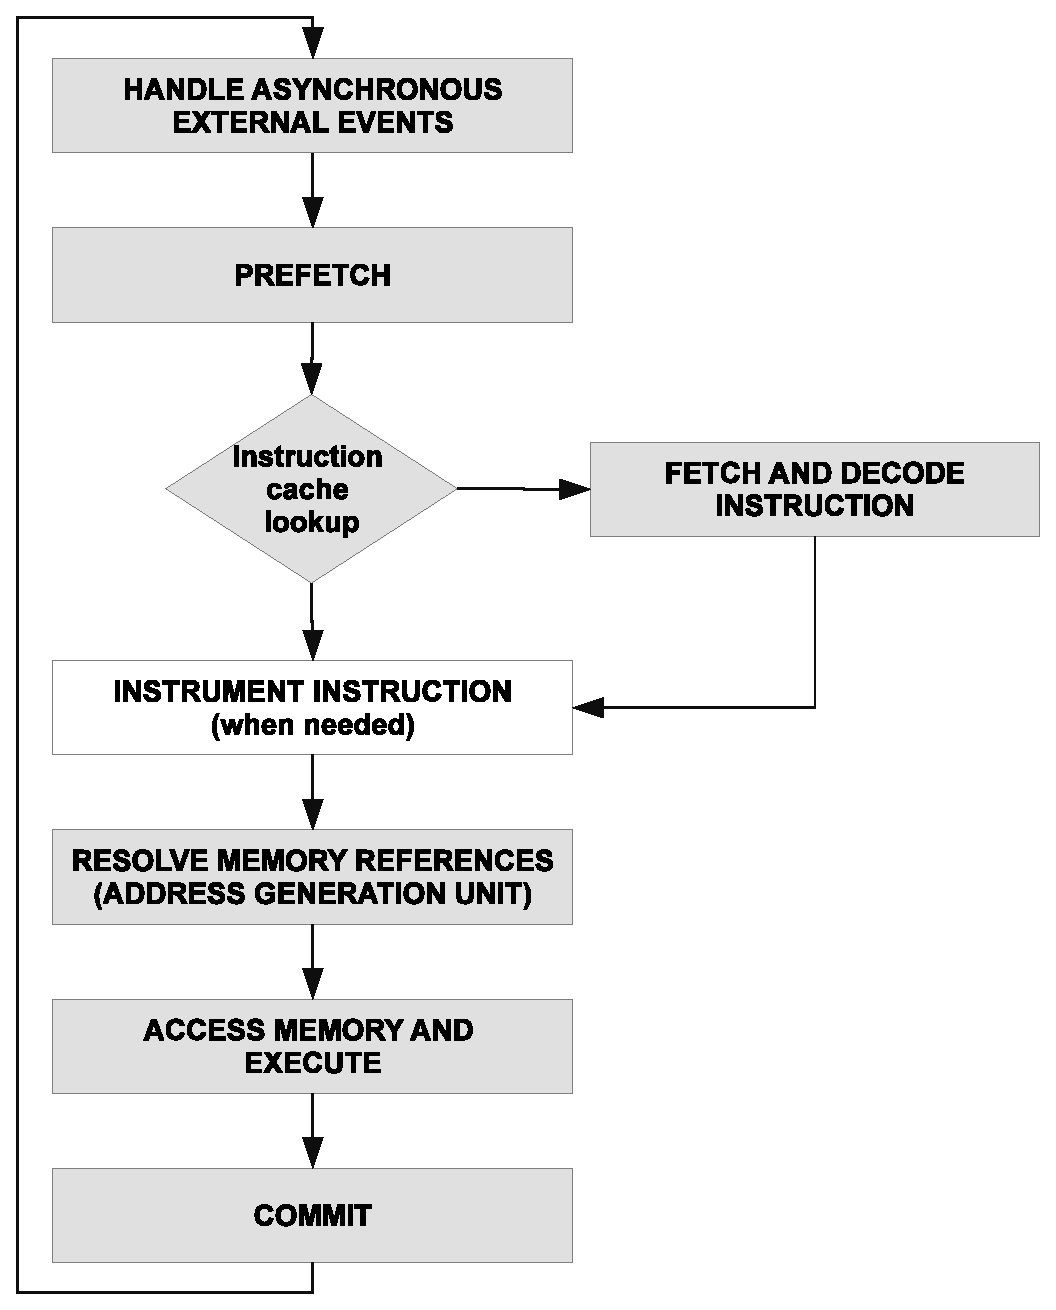
\includegraphics[scale=0.5]{figures/bochs_loop.eps}
	\end{center}
	\caption{Laço principal de interpretação de instruções do Bochs.}
	\label{fig:bochs_loop}
\end{figure}

\begin{itemize}
	\item \textbf{Events:} Nesse estágio ocorre a verificação se ocorreu
          alguma interrupção ou ``trap'' durante a interpretação da instrução
          anterior. Note que o Bochs possui suporte a execução de traços e
          threaded-interpretation. Essa verificação é feita apenas quando a
          execução volta ao laço principal de interpretação.

	\item \textbf{Prefetch:} Nesse estágio ocorre a verificação de
          permissões de acesso a página de código, validação de limites de
          segmento e o cálculo do endereço ``host'' da próxima instrução a ser
          emulada.

	\item \textbf{Decode:} Nesse estágio ocorre a busca e decodificação da
          instrução a ser emulada. O Bochs possui uma cache interna das
          instruções mais recentemente decodificadas. Se a instrução a ser
          interpretada estiver na cache, as informações são reutilizadas. Caso
          contrário, a instrução é decodificada.

	\item \textbf{Instrumentation:} Nesse estágio o Bochs verifica se a
          instrução a ser interpretada é alvo de alguma rotina de
          instrumentação. Em caso afirmativo, a rotina de instrumentação é
          invocada antes da interpretação da instrução.

	\item \textbf{Memory Addresses:} Nesse estágio, endereços de memória
          utilizados pela instrução a ser interpretada são resolvidos.  Em
          outras palavras, este passo é o responsável por tratar as várias
          formas de endereçamento presentes na família x86.

	\item \textbf{Execution:} Nesse estágio ocorre de fato a interpretação
          da instrução. Durante a decodificação da instrução, a rotina que deve
          efetuar a interpretação é anotada como meta-informação da
          instrução e este estágio utiliza essa informação para fazer
          uma chamada indireta para essa rotina.

	\item \textbf{Commit:} Esse estágio faz a consolidação da execução da
          instrução, isto é, atualiza o registrador EIP.

\end{itemize}


\subsection{Box}

Nesta seção descrevemos os principais componentes da máquina virtual de processo
Box e os maiores desafios enfrentados durante o seu desenvolvimento.

Como citado anteriormente, o desenvolvimento da máquina virtual de processos Box
baseou-se no código do Bochs, e embora ambas ainda compartilhem diversas
características em comum, principalmente relacionadas à interpretação de
instruções, ao final da implementação suas arquiteturas ficaram drasticamente
diferentes. Por exemplo, uma vez que o Bochs faz a execução de um sistema
operacional ele não precisa se preocupar com detalhes de criação de processos ou
chamadas de sistema, porém uma máquina de processos geralmente precisa. 

Da mesma forma, uma máquina virtual de processo não precisa emular dispositivos
como discos rígidos, placas de vídeo, rede, etc., uma vez que tais recursos não
são diretamente visíveis ao processo.

\subsubsection{Componentes Removidos}

Todos os componentes de hardware que não eram diretamente acessados pelos
processos foram removidos, isso inclui todo o subsistema de I/O e os
plugins específicos de dispositivos como placa de vídeo, placa de rede, placa de
som, mouse, teclado, cdrom, disco rígido, disquete, portas USB, barramento PCI,
COM, etc.

O subsistema de memória também sofreu grandes mudanças, pois originalmente o
Bochs emulava mecanismos de caches de instrução, dados e \emph{translation
lookaside buffer} (TLB). Todos esses recursos foram removidos por serem
transparentes ao processo durante a execução.

\subsubsection{Carregador}

A implementação do Box não conta com nenhum auxílio do sistema operacional para
preparar o ambiente de execução do processo sendo emulado. Por esse motivo, foi
necessário implementar mecanismos para permitir a emulação de toda a etapa de
carregamento e execução do processo. Isso trouxe uma série de complicações para
o desenvolvimento do projeto.

Não contar com o suporte do kernel significa que foi necessário implementar toda
a infraestrutura de código responsável por fazer o carregamento e ligação
dinâmica do executável principal e bibliotecas compartilhadas, bem como criar o
espaço de endereçamento e pilha de dados da aplicação.

Durante as etapas iniciais de desenvolvimento do projeto, o objetivo era o
desenvolvimento de um carregador suficientemente poderoso para suportar a
execução de aplicativos compilados com linkagem dinâmica utilizando a biblioteca
de runtime Glibc~\cite{glibc}. O carregador desenvolvido foi capaz de executar
pequenas aplicações com linkagem dinâmica, mas sem o uso da Glibc. Isso se deve
principalmente ao fato de que existem características que associam fortemente o
carregador à biblioteca de runtime, características das quais não fazem parte da
especificação da carga de executáveis ELF, previstas em \cite{SCO1997}.  Nesse
ponto percebemos que o desenvolvimento do carregador da forma inicialmente
proposta gastaria mais tempo que o disponível para a realização do projeto, e
dessa forma, foi decidido que no âmbito da avaliação proposta, o Box apenas iria
executar aplicações estaticamente compiladas utilizando a biblioteca
$\upmu$ClibC.

A principal tarefa do carregador atualmente implementado no Box é: 1) encontrar
o executável principal da aplicação; 2) fazer a leitura das estruturas do
executável (\emph{parsing}); 3) montar o espaço de endereçamento onde a
aplicação executará. A primeira tarefa é simples, uma vez que o usuário passa o
endereço completo da aplicação como parâmetro para o Box. O executável deve
estar codificado no formato ELF-32~\cite{SCO1997} e não fazer uso de linkagem
dinâmica. A segunda tarefa do carregador é fazer o parsing do executável e
encontrar quais segmentos (geralmente dois segmentos, um de texto e outro de
dados) de código devem ser carregados na memória. Uma vez que esses segmentos
tenham sido encontrados o carregador começa a montar o espaço de endereçamento
do processo. O espaço de endereçamento é montado seguindo a mesma estrutura que
seria utilizada pelo carregador nativo do Linux e é exemplificado na
Figura~\ref{fig:esp_end} para os casos com linkagem dinâmica e estática.

\begin{figure}[!h]
        \begin{center}
        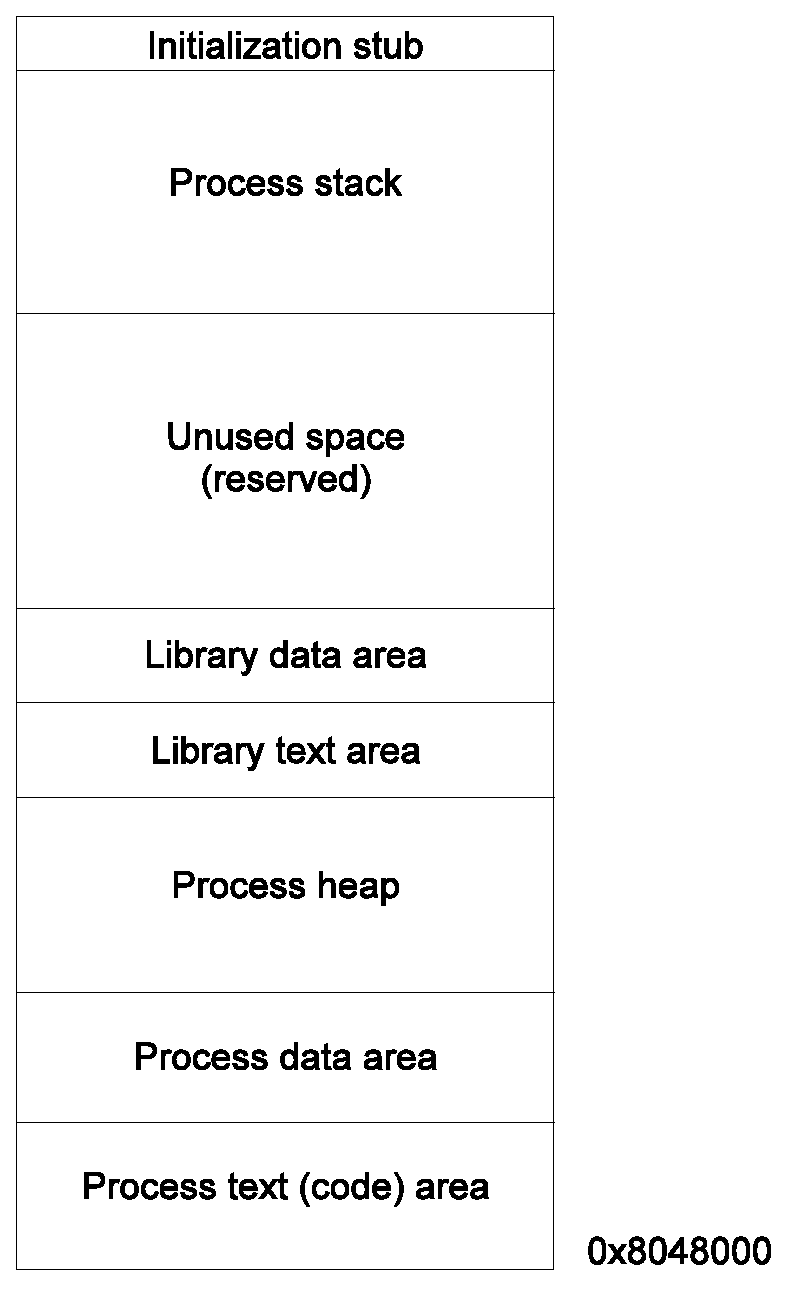
\includegraphics[scale=0.5]{figures/esp_end.eps}
        \end{center}
        \caption{Espaço de endereçamento inicial da aplicação.}
        \label{fig:esp_end}
\end{figure}

Outra tarefa desempenhada pelo kernel/carregador nativo do S.O. e que precisou ser
implementada no Box foi a criação da pilha de dados de execução da
aplicação. Além dos parâmetros e variáveis de ambiente a pilha inicial contém
informações que o kernel passa para o carregador nativo do sistema, estas
informações podem/são usadas tanto pelo carregador quanto pela biblioteca de
runtime utilizada. Essas informações são passadas na forma de um vetor e contém
dados como tamanho de página utilizado no sistema, endereço onde o
cabeçalho ELF do programa foi carregado, entre outras. A
Figura~\ref{fig:stack_ini} mostra o formato inicial da pilha de execução de um
programa.

\begin{figure}[!h]
  	\begin{center}
    	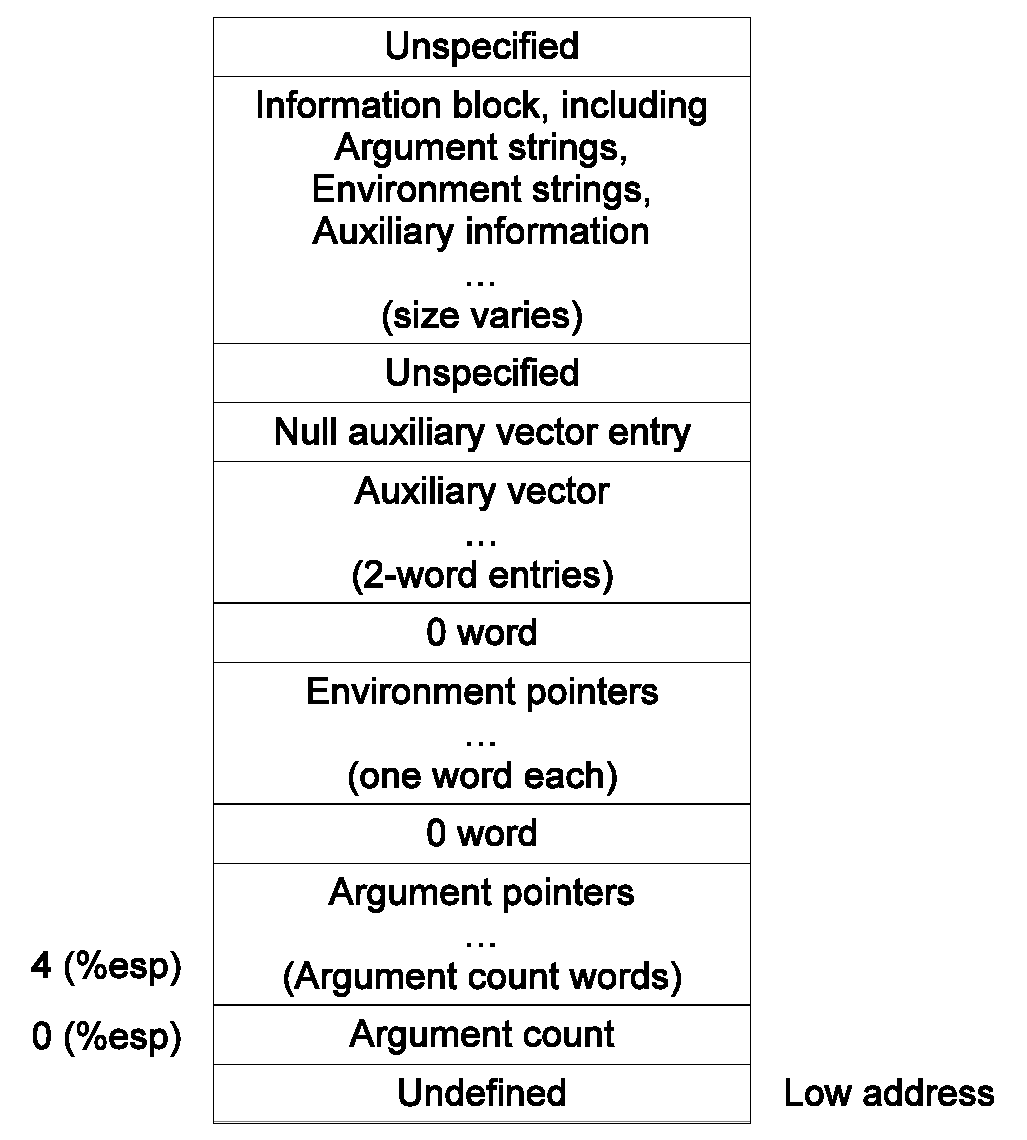
\includegraphics[scale=0.5]{figures/stack_ini.eps}
	\end{center}
	\caption{Formato da pilha inicial de execução de um programa.}
	\label{fig:stack_ini}
\end{figure}

\subsubsection{Emulação de Syscalls}

Sempre que a aplicação guest faz uma chamada ao sistema operacional o Box deve
interceptar essa chamada e decidir entre duas opções: 1) apenas ``redirecionar''
a chamada ao sistema nativo ou 2) implementar a execução da syscall. A
interceptação das chamadas é feita porque todas as instruções executadas pela
aplicação guest são interpretadas e porque pode ser necessária alguma tradução
dos endereços gerados pela aplicação.

Todas as instruções que não modificam o espaço de endereçamento da aplicação
guest são redirecionadas para o S.O. nativo. Exemplos de chamadas que são
tratadas dessa forma são: mkdir, fstat, getpid, getuid, uname, rename, rmdir,
nanosleep, utime, ioctl e chmod.

Aquelas chamadas de sistema que alteram o espaço de endereçamento da aplicação
ou que retornam informações que podem vir a ser usadas posteriormente para
controlar alguma alteração são implementadas pelo Box.  Exemplos de chamadas que
precisaram ser implementadas são: open, close, creat, brk, mmap e munmap. Estas
chamadas, com exceção da brk, estão relacionadas pelo fato de poderem ser
utilizadas para fazer ``\emph{memory mapped I/O}'', e portanto precisam de atenção
especial para fazer o mapeamento das entradas de dados diretamente para a
memória da aplicação sendo emulada. A chamada brk precisa ser implementada
porque ela é utilizada para aumentar o tamanho do segmento de dados do programa,
efetivamente sendo utilizada pela biblioteca de runtime para fazer requisição ao
S.O. para alocar mais memória para a aplicação.

O Box atualmente não conta com suporte para tratamento de sinais ou aplicações
que usam múltiplas threads de execução, portanto as chamadas de sistema
relacionadas a tais ações ainda não foram implementadas.

\subsubsection{Emulação da Memória}

O espaço de endereçamento da aplicação guest é totalmente independente do espaço
de endereçamento do Box. Atualmente o espaço de endereçamento guest é emulado
utilizando um vetor de tamanho fixo que pode ser configurado no momento de
compilação do Box.

Durante a inicialização do Box o carregador cria ponteiro para todos os
segmentos de memória que podem ser afetados durante a execução da aplicação.
Por exemplo, é criado um ponteiro para o primeiro byte após o segmento de dados
da aplicação, ponto conhecido como \emph{program break}, que aponta
para o primeiro byte do heap da aplicação. Quando chamadas para syscalls forem
tratadas, esse ponteiro será decrementado para aumentar o tamanho do segmento de
dados da aplicação. Outros ponteiros são criados para armazenar o início da
stack e os limites das regiões que contem código.

Também durante a inicialização do sistema o carregador registra o endereço
virtual base da aplicação. Isto é, em geral, o primeiro byte do segmento de
texto do executável principal. Esse endereço é associado com o primeiro byte do
vetor utilizado para emular a memória da aplicação guest, e a partir de então
todos os acessos a memória são traduzidos utilizando esse endereço base.

O Box atualmente não trata proteção de páginas.

\subsection{Mibench}

\begin{table}                                                                                                                                                                                              
 \caption{Número de instruções e syscalls dos aplicativos do MiBench}
 \begin{center}
  \begin{tabular}{|l|r|r|} \hline
    \bf{Aplicativo} & \bf{Instruções} & \bf{Syscalls} \\ \hline                                                                                                                                            
    basichmath & 2245174977 & 7996 \\ \hline
    bitcount & 645799557 & 18 \\ \hline
    qsort & 724781929 & 1160 \\ \hline
    susan-smoothing & 26107053 & 19 \\ \hline
    susan-edges & 62382631 & 20 \\ \hline
    susan-corners & 19305482 & 23 \\ \hline
    tiff2rgba & 133523722 & 12455 \\ \hline
    tiffmedian & 544600121 & 15583 \\ \hline
    tiffdither & 904052825 & 3471 \\ \hline
    tiff2bw & 154051379 & 9353 \\ \hline
    cjpeg & 84673918 & 542 \\ \hline
    djpeg & 23591372 & 365 \\ \hline
    patricia & 531614551 & 2050 \\ \hline
    dijkstra & 186205562 & 1096 \\ \hline
    ispell & 778996260 & 6957 \\ \hline
    search & 8859144 & 47 \\ \hline
    say & 95772915 & 64 \\ \hline
    blowfish-e & 625506759 & 1600 \\ \hline
    blowfish-d & 635168355 & 1600 \\ \hline
    rijndael-e & 233325816 & 204569 \\ \hline
    rijndael-d & 233732135 & 204567 \\ \hline
    sha & 123886774 & 408 \\ \hline
    pgp-sa & 6825231 & 340 \\ \hline
    pgp-z & 13567840 & 5781 \\ \hline
    rawcaudio & 729304831 & 26622 \\ \hline
    rawdaudio & 682210259 & 26622 \\ \hline
    crc32 & 985166454 & 6508 \\ \hline
    toast & 2063665205 & 412 \\ \hline
    untoast & 807954820 & 7539 \\ \hline
  \end{tabular}
  \label{tab:mibench}
 \end{center}
\end{table}

A infraestrutura de testes, em relação a benchmarks, que utilizamos durante o
desenvolvimento e medição de desempenho do sistema é baseada no conjunto de
aplicativos Mibench~\cite{mibench}. O Mibench contém vários aplicativos
divididos em seis grupos: automotivo, rede, escritório, telecomunicações,
segurança e entretenimento. O Mibench foi projetado para testes de sistemas
embarcados e para tanto os aplicativos que o compõe em geral são pequenos (em
código estático), possuem um pequeno foot print dinâmico (número de instruções
tocadas durante a execução) e tem um curto período de execução. A 
Tabela~\ref{tab:mibench} mostra algumas informações sobre o Mibench que 
coletamos durante nossos experimentos.

Nossa escolha por este conjunto de aplicações é principalmente devido ao curto
período de execução das aplicações. Consideramos utilizar outros conjuntos de
programas para teste, como por exemplo o SPEC CPU 2006~\cite{spec2006}, porém
para testar a primeira versão do sistema resolvemos começar com programas mais
``simples''.

\subsection{$\upmu$ClibC}

Uma das etapas que mais gastou tempo de desenvolvimento no Box foi a parte de
configuração do ambiente de inicialização do programa/libc.  Grande parte dessa
dificuldade é devido a falta de documentação explicando de forma clara qual é a
parte do kernel e do loader na tarefa de criação de processos no
Linux. Especificamente, é difícil encontrar literatura dizendo qual seria o
estado dos registradores e qual a estrutura do espaço de endereçamento no
momento em que o processo é inicializado. Para resolver essa falta de
documentação tivemos que inspecionar diretamente o código do Linux, porém isso
retardou o processo de desenvolvimento do Box e a decisão de não utilizar a
Glibc e linkagem dinâmica foi tomada.

A $\upmu$ClibC é uma biblioteca C desenvolvida com o propósito de rodar em
sistemas Linux para dispositivos embarcados. Dessa forma ela é bem menos
genérica que a Glibc e por isso possui um \emph{foot print} de execução bem
menor. Outra característica importante da $\upmu$ClibC é a possibilidade de
fazer sua instalação de forma seletiva de seus componentes. Estas e outras
características nos levaram a escolher a $\upmu$ClibC como alternativa a GlibC.

Como a implementação atual do Box não possui suporte a \emph{multithreading}, a
instalação da $\upmu$ClibC que utilizamos nos testes não consta com estes
recurso.


\section{Resultados} \label{sec:resultados}

Nessa seção apresentamos os resultados que obtivemos nos nossos experimentos
com o Box e Bochs. Inicialmente apresentamos a metodologia que seguimos para
os testes, em seguida apresentamos os resultados da comparação do Box com o
Bochs e a execução nativa, e posteriormente mostramos o ganho de desempenho com
a introdução da cache de decodificação, DICache, no Box. 
%Por fim apresentamos
%uma análise mostrando quais componentes do Box dominam o tempo de execução de
%diversos benchmarks.

\subsection{Metodologia}

Todos os experimentos foram realizados em uma máquina de 32 bits rodando o
sistema operacional Debian Squeeze. A máquina de testes é um Intel Core 2 Duo
de 2.13 GHz, com 4Mb de cache L2 e 3Gb de memória RAM.

Os aplicativos utilizados para testes são os presentes no benchmark Mibench. Nos
experimentos rodamos os programas com as entradas ``pequenas'' e ``grandes'',
aqui mostramos apenas os gráficos para a entrada grande. O Apêndice A contém
os resultados em forma de tabela para todos os benchmarks.

Os experimentos foram feitos na máquina em modo mono-usuário (\textit{runlevel
  1}) e para cada par aplicativo/entrada foi coletado o tempo de dez execuções,
aqui mostramos apenas a média arimética destas dez execuções. O Apêndice A
contém os valores de intervalo de confiança e desvio padrão, os quais omitimos
aqui porquê, como pode ser visto no apêndice, a margem de erro e o desvio padrão
foram desprezíveis.

Utilizamos o Bochs-2.6 nos experimentos, atualmente esta é a versão mais recente.


\subsection{Overhead de Emulação de Sistema}

A Figura~\ref{fig:bochs_nocache_nativo} apresenta os tempos de execução dos 
aplicativos do Mibench executados nativamente, no Bochs e no Box sem nenhum 
tipo de otimização. De modo geral, a comparação entre os tempos de execução das 
máquinas virtuais de sistema e processo mostrou que a versão de sistema apresentou 
tempos significativamente menores. Tal diferença pode ser justificada pelo fato do
Bochs contar com otimizações que são direcionadas à implementação do subsistema de 
memória e a utilização da cache de instruções pré decodificadas. Os resultados 
indicam que essas otimizações foram suficientes para superar qualquer redução de 
tempo obtido pela eliminação de emulação da parte de sistema operacional. 

\begin{figure}[h]
	\centering
	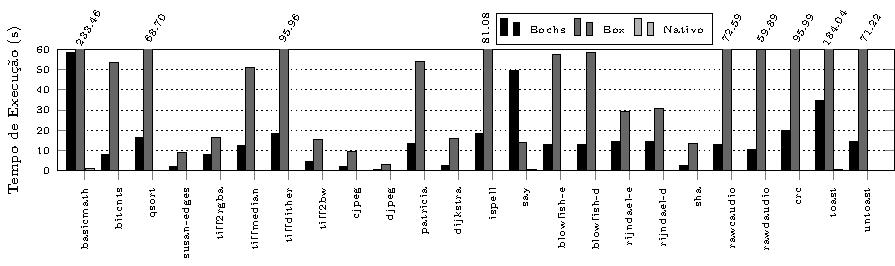
\includegraphics[width=1.0\textwidth]{figures/bochs_nocache_nativo}
	\caption{Tempo de execução do Mibench no Bochs, Box e nativamente.}
	\label{fig:bochs_nocache_nativo}
\end{figure}

Através dos resultados obtidos é possível observar o impacto causado pela
decodificação contínua de instruções (usada pelo Box) comparada com a 
abordagem de pré decodificação utilizada pelo Bochs.

\subsection{Otimizando a Interpretação}

Como forma de minimizar o impacto causado pela decodificação repetida de
instruções já executada, duas abordagens foram adotadas. Na primeira, foi
implementada a técnica DICache \cite{dicache}, na segunda, o código de
pré decodificação de instruções do Bochs foi incluído no Box. Para isso
modificações tiveram que ser feitas no código original do Bochs para garantir a
compatibilidade com o subsistema de memória utilizado no Box. Alterações também
foram necessárias no laço de interpretação de instruções do Box de modo a
integrar a novas funcionalidade. A Figura~\ref{fig:dicache_nocache} apresenta os
resultados obtidos com a implementação das duas abordagens.

\begin{figure}[h]
	\centering
	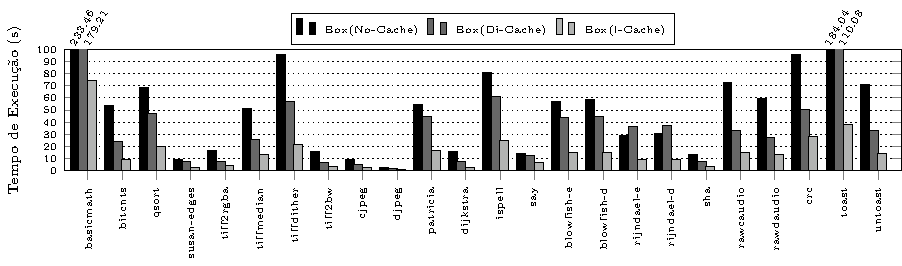
\includegraphics[width=1.0\textwidth]{figures/dicache_nocache}
	\caption{Tempo de execução do Mibench no Box com DICache, I-Cache e sem cache.}
	\label{fig:dicache_nocache}
\end{figure}

Pode-se observar que alguns aplicativos tiveram uma redução significativa no
tempo de execução. Conforme apresentado na Figura~\ref{fig:bochs_icache}, a
implementação da código de emulação do cache de instruções em algumas casos
resultou em tempos de execução inferiores aos tempos de execução na máquina
virtual de sistemas.

É importante destacar que as otimizações empregadas foram executadas de forma
exclusiva, pois não foi possível dentro do prazo disponível implementar as
modificações necessárias para permitir que ambas fosse utilizadas em conjunto.

\begin{figure}[h]
        \centering
        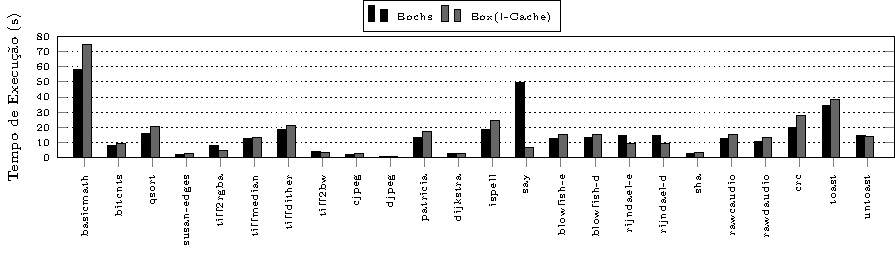
\includegraphics[width=1.0\textwidth]{figures/bochs_icache}
        \caption{Tempos de execução do Mibench no Bochs e Box com cache de instruções.}
        \label{fig:bochs_icache}
\end{figure}

\section{Conclusões} \label{sec:conclusao}

Este relatório apresentou as descobertas encontradas durante a análise
comparativa entre máquinas virtuais de sistema e de processo.  Para a realização
desta análise, foi desenvolvida uma máquina virtual de processos interpretada
para execução de aplicativos Linux IA-32, baseado no código da máquina virtual
de sistema Bochs.  
Os resultados obtidos nos testes não sustentaram a hipótese da
existência de \emph{overhead} causado pela interpretação de todo o sistema operacional
em máquinas virtuais de sistema. Tal fato pode ser justificado pelos seguintes
fatores:

\begin{itemize}
 \item Não foi possível desativar totalmente as otimizações existentes no Bochs,
   visto que muitas delas estão fortemente associadas a subsistemas que integram
   a máquina virtual;
 \item Em condições normais, a execução de um sistema operacional deve produzir
   um baixo impacto no tempo de execução da aplicação, uma vez que na maior parte do tempo o código em execução é da aplicação, e não do sistema operacional.
\end{itemize}

Embora não tenha sido possível provar a existência de \emph{overhead} de
execução de máquinas virtuais de sistema, foi comprovado o impacto causado pela
aplicação de técnicas de otimização em uma MV. A redução no tempo
de execução das aplicações executada no Box utilizando otimizações mostra o
quanto a interpretação pode ser beneficiada com a utilização de técnicas de
otimização como DICache e pré-decodificação.

Os resultados obtidos nos testes com otimização mostram que a MV desenvolvida
tem potencial para executar aplicações com tempos inferiores aos tempos de uma
MV de sistema. Essa característica, aliada ao fato de que MVs de processos
possuem menos requisitos necessários para a execução de programa, transforma o
Box numa poderosa ferramenta para teste e análise de execução de
aplicativos. Para isso, estão previstos como trabalhos futuros:

\begin{itemize}
	\item Aprimorar o subsistema de memória, melhorando o controle de segmentação e fornecendo suporte a paginação de memória.
        \item Implementação de suporte a execução carregadores externos (não pertencente ao Box).
	\item Implementação de novas chamadas de sistema (\emph{syscalls}).
	\item Implementação de mecanismos de instrumentação de código.
	\item Suporte a execução em diferentes plataformas e ou sistemas operacionais.
\end{itemize}

\newpage

\section*{Apêndice A} \label{ap:results}

As Tabelas~\ref{tab:tempos_medios} à \ref{tab:tempos_boxicache} mostram os 
resultados que obtivemos com o conjunto de aplicativos Mibench executando a 
entrada de dados grande. Os resultados apresentados são derivados de 10 
execuções de cada benchmark/entrada.

\begin{table}[!h]
 \caption{Tempo médio de execução nativa, Box-NoCache, Box-DiCache, Bochs e Box-ICache.}
 \begin{center}
 \begin{tabular}{|l|r|r|r|}
        \bf{Benchmark} & \bf{Nativo} & \bf{NoCache} & \bf{DiCache} & \bf{Bochs}  & \bf{ICache} \\ \hline
        basicmath & 1.023 & 233.463 & 179.211 & 58.402 & 74.511\\ \hline
        bitcnts & 0.183 & 53.376 & 23.985 & 8.277 & 9.332\\ \hline
        qsort & 0.250 & 68.704 & 46.879 & 16.224 & 20.299\\ \hline
        susan-smoothing & 0.134 & 3.374 & 1.617 & 11.175 & 0.983\\ \hline
        susan-edges & 0.037 & 9.182 & 7.627 & 1.904 & 2.558\\ \hline
        susan-corners & 0.012 & 2.823 & 2.044 & 0.653 & 0.803\\ \hline
        tiff2rgba & 0.335 & 16.606 & 7.887 & 8.053 & 4.701\\ \hline
        tiffmedian & 0.278 & 50.930 & 25.397 & 12.389 & 13.447\\ \hline
        tiffdither & 0.280 & 95.966 & 57.333 & 18.348 & 21.579\\ \hline
        tiff2bw & 0.085 & 15.562 & 6.925 & 4.331 & 3.713\\ \hline
        cjpeg & 0.050 & 9.294 & 4.845 & 2.003 & 2.525\\ \hline
        djpeg & 0.017 & 2.964 & 1.746 & 0.777 & 0.921\\ \hline
        patricia & 0.222 & 54.226 & 44.347 & 13.230 & 17.006\\ \hline
        dijkstra & 0.057 & 15.967 & 7.686 & 2.809 & 2.968\\ \hline
        ispell & 0.301 & 81.081 & 60.786 & 18.511 & 24.859\\ \hline
        search & 0.010 & 0.859 & 0.636 & 0.238 & 0.279\\ \hline
        say & 0.823 & 14.113 & 12.151 & 49.562 & 6.946\\ \hline
        blowfish-e & 0.196 & 57.234 & 44.264 & 12.952 & 15.022\\ \hline
        blowfish-d & 0.197 & 58.386 & 44.707 & 13.045 & 15.157\\ \hline
        rijndael-e & 0.266 & 29.349 & 36.451 & 14.557 & 9.246\\ \hline
        rijndael-d & 0.254 & 30.866 & 37.343 & 14.636 & 9.442\\ \hline
        sha & 0.042 & 13.453 & 7.723 & 2.571 & 3.602\\ \hline
        pgp-sa & 0.051 & 0.670 & 0.447 & 0.231 & 0.286\\ \hline
        pgp-z & 0.039 & 1.220 & 0.714 & 0.361 & 0.445\\ \hline
        rawcaudio & 0.339 & 72.592 & 33.437 & 12.855 & 15.301\\ \hline
        rawdaudio & 0.279 & 59.891 & 27.648 & 10.383 & 13.387\\ \hline
        crc & 0.305 & 95.995 & 50.293 & 20.076 & 27.880\\ \hline
        toast & 0.501 & 184.047 & 110.080 & 34.731 & 38.157\\ \hline
        untoast & 0.228 & 71.222 & 33.199 & 14.685 & 14.171\\ \hline
  \end{tabular}
  \label{tab:tempos_medios}
 \end{center}
\end{table}

\begin{table}
 \caption{Tempo médio de execução nativa, desvio padrão e intervalo de confiança.}
 \begin{center}
 \begin{tabular}{|l|r|r|r|}
   \cline{2-4}
   \multicolumn{1}{c|}{}& \multicolumn{3}{|c|}{Nativo} \\ \hline
   \bf{Benchmark} & \bf{Média} & \bf{Desvio Padrão} & \bf{Int. de Confiança} \\ \hline
   basicmath & 1.023 & 0.002 & 0.001\\ \hline
   bitcnts & 0.183 & 0.011 & 0.007\\ \hline
   qsort & 0.250 & 0.020 & 0.012\\ \hline
   susan-smoothing & 0.134 & 0.022 & 0.014\\ \hline
   susan-edges & 0.037 & 0.006 & 0.004\\ \hline
   susan-corners & 0.012 & 0.005 & 0.003\\ \hline
   tiff2rgba & 0.335 & 0.218 & 0.135\\ \hline
   tiffmedian & 0.278 & 0.020 & 0.013\\ \hline 
   tiffdither & 0.280 & 0.028 & 0.018\\ \hline 
   tiff2bw & 0.085 & 0.012 & 0.007\\ \hline 
   cjpeg & 0.050 & 0.053 & 0.033\\ \hline 
   djpeg & 0.017 & 0.011 & 0.007\\ \hline 
   patricia & 0.222 & 0.023 & 0.014\\ \hline 
   dijkstra & 0.057 & 0.013 & 0.008\\ \hline 
   ispell & 0.301 & 0.034 & 0.021\\ \hline 
   search & 0.010 & 0.017 & 0.010\\ \hline 
   say & 0.823 & 0.022 & 0.013\\ \hline 
   blowfish-e & 0.196 & 0.034 & 0.021\\ \hline 
   blowfish-d & 0.197 & 0.011 & 0.007\\ \hline 
   rijndael-e & 0.266 & 0.019 & 0.011\\ \hline 
   rijndael-d & 0.254 & 0.002 & 0.001\\ \hline 
   sha & 0.042 & 0.025 & 0.015\\ \hline 
   pgp-sa & 0.051 & 0.056 & 0.035\\ \hline 
   pgp-z & 0.039 & 0.015 & 0.009\\ \hline 
   rawcaudio & 0.339 & 0.130 & 0.081\\ \hline 
   rawdaudio & 0.279 & 0.013 & 0.008\\ \hline 
   crc & 0.305 & 0.010 & 0.006\\ \hline 
   toast & 0.501 & 0.023 & 0.014\\ \hline 
   untoast & 0.228 & 0.006 & 0.004 \\
   \hline
  \end{tabular}
  \label{tab:tempos_nativo}
 \end{center}
\end{table}

\begin{table}
 \caption{Tempo médio de execução no Box-NoCache, desvio padrão e intervalo de confiança.}
 \begin{center}
 \begin{tabular}{|l|r|r|r|}
   \cline{2-4}
   \multicolumn{1}{c|}{}& \multicolumn{3}{|c|}{Box-NoCache} \\ \hline
   \bf{Benchmark} & \bf{Média} & \bf{Desvio Padrão} & \bf{Int. de Confiança} \\ \hline
   basicmath & 233.463 & 3.716 & 2.303\\ \hline 
   bitcnts & 53.376 & 0.238 & 0.148\\ \hline 
   qsort & 68.704 & 0.483 & 0.299\\ \hline 
   susan-smoothing & 3.374 & 0.047 & 0.029\\ \hline 
   susan-edges & 9.182 & 0.042 & 0.026\\ \hline 
   susan-corners & 2.823 & 0.028 & 0.017\\ \hline 
   tiff2rgba & 16.606 & 0.054 & 0.034\\ \hline 
   tiffmedian & 50.930 & 0.526 & 0.326\\ \hline 
   tiffdither & 95.966 & 0.781 & 0.484\\ \hline 
   tiff2bw & 15.562 & 0.602 & 0.373\\ \hline 
   cjpeg & 9.294 & 0.022 & 0.014\\ \hline 
   djpeg & 2.964 & 0.026 & 0.016\\ \hline 
   patricia & 54.226 & 0.578 & 0.358\\ \hline 
   dijkstra & 15.967 & 0.194 & 0.120\\ \hline 
   ispell & 81.081 & 0.610 & 0.378\\ \hline 
   search & 0.859 & 0.044 & 0.027\\ \hline 
   say & 14.113 & 0.024 & 0.015\\ \hline 
   blowfish-e & 57.234 & 0.489 & 0.303\\ \hline 
   blowfish-d & 58.386 & 0.436 & 0.271\\ \hline 
   rijndael-e & 29.349 & 0.160 & 0.099\\ \hline 
   rijndael-d & 30.866 & 1.935 & 1.199\\ \hline 
   sha & 13.453 & 0.089 & 0.055\\ \hline 
   pgp-sa & 0.670 & 0.002 & 0.001\\ \hline 
   pgp-z & 1.220 & 0.011 & 0.007\\ \hline 
   rawcaudio & 72.592 & 0.549 & 0.340\\ \hline 
   rawdaudio & 59.891 & 0.314 & 0.194\\ \hline 
   crc & 95.995 & 1.538 & 0.953\\ \hline 
   toast & 184.047 & 1.334 & 0.827\\ \hline 
   untoast & 71.222 & 0.718 & 0.445\\
   \hline
  \end{tabular}
  \label{tab:tempos_boxnocache}
 \end{center}
\end{table}
 
\begin{table}
 \caption{Tempo médio de execução no Box-DiCache, desvio padrão e intervalo de confiança.}
 \begin{center}
 \begin{tabular}{|l|r|r|r|}
   \cline{2-4}
   \multicolumn{1}{c|}{}& \multicolumn{3}{|c|}{Box-DiCache} \\ \hline
   \bf{Benchmark} & \bf{Média} & \bf{Desvio Padrão} & \bf{Int. de Confiança} \\ \hline
   basicmath & 179.211 & 0.474 & 0.294\\ \hline 
   bitcnts & 23.985 & 0.075 & 0.046\\ \hline 
   qsort & 46.879 & 0.352 & 0.218\\ \hline 
   susan-smoothing & 1.617 & 0.034 & 0.021\\ \hline 
   susan-edges & 7.627 & 0.019 & 0.012\\ \hline 
   susan-corners & 2.044 & 0.006 & 0.003\\ \hline 
   tiff2rgba & 7.887 & 0.124 & 0.077\\ \hline 
   tiffmedian & 25.397 & 0.313 & 0.194\\ \hline 
   tiffdither & 57.333 & 0.087 & 0.054\\ \hline 
   tiff2bw & 6.925 & 0.034 & 0.021\\ \hline 
   cjpeg & 4.845 & 0.028 & 0.017\\ \hline 
   djpeg & 1.746 & 0.021 & 0.013\\ \hline 
   patricia & 44.347 & 0.139 & 0.086\\ \hline 
   dijkstra & 7.686 & 0.011 & 0.007\\ \hline 
   ispell & 60.786 & 0.078 & 0.048\\ \hline 
   search & 0.636 & 0.004 & 0.002\\ \hline 
   say & 12.151 & 0.045 & 0.028\\ \hline 
   blowfish-e & 44.264 & 0.413 & 0.256\\ \hline 
   blowfish-d & 44.707 & 0.405 & 0.251\\ \hline 
   rijndael-e & 36.451 & 0.106 & 0.066\\ \hline 
   rijndael-d & 37.343 & 0.222 & 0.137\\ \hline 
   sha & 7.723 & 0.086 & 0.053\\ \hline 
   pgp-sa & 0.447 & 0.002 & 0.001\\ \hline 
   pgp-z & 0.714 & 0.004 & 0.002\\ \hline 
   rawcaudio & 33.437 & 0.295 & 0.183\\ \hline 
   rawdaudio & 27.648 & 0.281 & 0.174\\ \hline 
   crc & 50.293 & 0.555 & 0.344\\ \hline 
   toast & 110.080 & 0.884 & 0.548\\ \hline 
   untoast & 33.199 & 0.097 & 0.060\\
   \hline
  \end{tabular}
  \label{tab:tempos_boxdicache}
 \end{center}
\end{table}

\begin{table}
 \caption{Tempo médio de execução no Bochs, desvio padrão e intervalo de confiança.}
 \begin{center}
 \begin{tabular}{|l|r|r|r|}
   \cline{2-4}
   \multicolumn{1}{c|}{}& \multicolumn{3}{|c|}{Bochs} \\ \hline
   \bf{Benchmark} & \bf{Média} & \bf{Desvio Padrão} & \bf{Int. de Confiança} \\ \hline
   basicmath & 58.402 & 0.106 & 0.066\\ \hline 
   bitcnts & 8.277 & 0.019 & 0.012\\ \hline 
   qsort & 16.224 & 0.103 & 0.064\\ \hline 
   susan-smoothing & 11.175 & 0.766 & 0.474\\ \hline 
   susan-edges & 1.904 & 0.013 & 0.008\\ \hline 
   susan-corners & 0.653 & 0.025 & 0.016\\ \hline 
   tiff2rgba & 8.053 & 0.483 & 0.299\\ \hline 
   tiffmedian & 12.389 & 0.740 & 0.458\\ \hline 
   tiffdither & 18.348 & 0.120 & 0.075\\ \hline 
   tiff2bw & 4.331 & 0.137 & 0.085\\ \hline 
   cjpeg & 2.003 & 0.099 & 0.062\\ \hline 
   djpeg & 0.777 & 0.010 & 0.006\\ \hline 
   patricia & 13.230 & 0.105 & 0.065\\ \hline 
   dijkstra & 2.809 & 0.012 & 0.008\\ \hline 
   ispell & 18.511 & 0.893 & 0.553\\ \hline 
   search & 0.238 & 0.010 & 0.006\\ \hline 
   say & 49.562 & 0.052 & 0.032\\ \hline 
   blowfish-e & 12.952 & 0.070 & 0.043\\ \hline 
   blowfish-d & 13.045 & 0.057 & 0.036\\ \hline 
   rijndael-e & 14.557 & 0.260 & 0.161\\ \hline 
   rijndael-d & 14.636 & 0.266 & 0.165\\ \hline 
   sha & 2.571 & 0.030 & 0.018\\ \hline 
   pgp-sa & 0.231 & 0.030 & 0.019\\ \hline 
   pgp-z & 0.361 & 0.007 & 0.005\\ \hline 
   rawcaudio & 12.855 & 0.252 & 0.156\\ \hline 
   rawdaudio & 10.383 & 0.071 & 0.044\\ \hline 
   crc & 20.076 & 0.101 & 0.062\\ \hline 
   toast & 34.731 & 0.177 & 0.109\\ \hline 
   untoast & 14.685 & 5.718 & 3.544\\
   \hline
 \end{tabular}
 \label{tab:tempos_bochs}
 \end{center}
\end{table}

\begin{table}
 \caption{Tempo médio de execução no Box-ICache, desvio padrão e intervalo de confiança.}
 \begin{center}
 \begin{tabular}{|l|r|r|r|}
   \cline{2-4}
   \multicolumn{1}{c|}{}& \multicolumn{3}{|c|}{Box-ICache} \\ \hline
   \bf{Benchmark} & \bf{Média} & \bf{Desvio Padrão} & \bf{Int. de Confiança} \\ \hline
   basicmath & 74.511 & 0.303 & 0.188\\ \hline 
   bitcnts & 9.332 & 0.058 & 0.036\\ \hline 
   qsort & 20.299 & 0.062 & 0.039\\ \hline 
   susan-smoothing & 0.983 & 0.005 & 0.003\\ \hline 
   susan-edges & 2.558 & 0.019 & 0.012\\ \hline 
   susan-corners & 0.803 & 0.010 & 0.006\\ \hline 
   tiff2rgba & 4.701 & 0.392 & 0.243\\ \hline 
   tiffmedian & 13.447 & 0.142 & 0.088\\ \hline 
   tiffdither & 21.579 & 0.061 & 0.038\\ \hline 
   tiff2bw & 3.713 & 0.027 & 0.017\\ \hline 
   cjpeg & 2.525 & 0.011 & 0.007\\ \hline 
   djpeg & 0.921 & 0.025 & 0.015\\ \hline 
   patricia & 17.006 & 0.071 & 0.044\\ \hline 
   dijkstra & 2.968 & 0.022 & 0.014\\ \hline 
   ispell & 24.859 & 0.038 & 0.024\\ \hline 
   search & 0.279 & 0.003 & 0.002\\ \hline 
   say & 6.946 & 0.038 & 0.024\\ \hline 
   blowfish-e & 15.022 & 0.301 & 0.187\\ \hline 
   blowfish-d & 15.157 & 0.095 & 0.059\\ \hline 
   rijndael-e & 9.246 & 0.016 & 0.010\\ \hline 
   rijndael-d & 9.442 & 0.080 & 0.049\\ \hline 
   sha & 3.602 & 0.031 & 0.019\\ \hline 
   pgp-sa & 0.286 & 0.003 & 0.002\\ \hline 
   pgp-z & 0.445 & 0.004 & 0.003\\ \hline 
   rawcaudio & 15.301 & 0.067 & 0.042\\ \hline 
   rawdaudio & 13.387 & 1.041 & 0.645\\ \hline 
   crc & 27.880 & 0.252 & 0.156\\ \hline 
   toast & 38.157 & 0.110 & 0.068\\ \hline 
   untoast & 14.171 & 0.072 & 0.045\\
   \hline
 \end{tabular}
 \label{tab:tempos_boxicache}
 \end{center}
\end{table}

\newpage

\bibliography{box}

\end{document}
